\ifdefined\ishandout
\documentclass[handout]{beamer}
\else
\documentclass{beamer}
\fi

\usepackage[frenchb]{babel}
\usepackage[T1]{fontenc}
\usepackage[latin1]{inputenc}
\usepackage{hyperref}
\usepackage{multirow}
\usepackage{listings}
\usepackage{fancyvrb}
\usepackage{tikz}
\usepackage{framed}
\usepackage{algorithm}
\usepackage{algorithmic}
\usepackage{xcolor}
\usepackage{color, colortbl}
\ifdefined\ishandout
\usepackage{handoutWithNotes}
\fi
\usepackage{slashbox}
\usepackage{amsmath}
\usepackage{bm}
\usepackage{hhline}

\usetikzlibrary{shapes.geometric}
\usetikzlibrary{positioning}
\usetikzlibrary{shapes.arrows, chains}
\usetikzlibrary{arrows,calc}
\usetikzlibrary{shapes.multipart}
\usepackage{array}
\usetheme{Boadilla}

\usefonttheme[onlymath]{serif}

\newcommand{\R}{\mathbb{R}}
\newcommand{\C}{\mathbb{C}}
\newcommand{\N}{\mathbb{N}}
\newcommand{\Z}{\mathbb{Z}}


\ifdefined\ishandout
\pgfpagesuselayout{3 on 1 with notes}[a4paper,border shrink=5mm]
\usecolortheme{dove}
\else
%\usecolortheme{dolphin}
\usecolortheme{beaver}
\fi


\lstnewenvironment{codeC}
{ \lstset{language=C,
    otherkeywords={printf,scanf}}
}
{}

\ifdefined\ishandout
\definecolor{mygreen}{rgb}{0,0,0}
\definecolor{mymauve}{rgb}{0,0,0}
\definecolor{myblue}{rgb}{0,0,0}
\else
\definecolor{mygreen}{rgb}{0,0.6,0}
\definecolor{mymauve}{rgb}{0.58,0,0.82}
\definecolor{myblue}{rgb}{0,0,1}

\fi

%% Notes
%\setbeameroption{show only notes}


\definecolor{mygray}{rgb}{0.5,0.5,0.5}

\lstset{ language=Python,%
  backgroundcolor=\color{white},   % choose the background color; you must add \usepackage{color} or \usepackage{xcolor}
  basicstyle=\footnotesize,        % the size of the fonts that are used for the code
  breakatwhitespace=false,         % sets if automatic breaks should only happen at whitespace
  breaklines=true,                 % sets automatic line breaking
  captionpos=b,                    % sets the caption-position to bottom
  commentstyle=\color{mygreen},    % comment style
  deletekeywords={...},            % if you want to delete keywords from the given language
  escapeinside={\%*}{*)},          % if you want to add LaTeX within your code
  extendedchars=true,              % lets you use non-ASCII characters; for 8-bits encodings only, does not work with UTF-8
  frame=tb,	                   % adds a frame around the code
  keepspaces=true,                 % keeps spaces in text, useful for keeping indentation of code (possibly needs columns=flexible)
  keywordstyle=\color{blue},       % keyword style
  otherkeywords={*,...},           % if you want to add more keywords to the set
  numbers=none,                    % where to put the line-numbers; possible values are (none, left, right)
  numbersep=5pt,                   % how far the line-numbers are from the code
  numberstyle=\tiny\color{mygray}, % the style that is used for the line-numbers
  rulecolor=\color{black},         % if not set, the frame-color may be changed on line-breaks within not-black text (e.g. comments (green here))
  showspaces=false,                % show spaces everywhere adding particular underscores; it overrides 'showstringspaces'
  showstringspaces=false,          % underline spaces within strings only
  showtabs=false,                  % show tabs within strings adding particular underscores
  stepnumber=2,                    % the step between two line-numbers. If it's 1, each line will be numbered
  stringstyle=\color{mymauve},     % string literal style
  tabsize=3,	                   % sets default tabsize to 2 spaces
  title=\lstname                   % show the filename of files included with \lstinputlisting; also try caption instead of title
}
%\lstset{language=Python,
% breakatwhitespace=false,         % sets if automatic breaks should only happen at whitespace
%  breaklines=true,                 % sets automatic line breaking
%  captionpos=b,                
%%commentstyle=\itshape\color{mymauve},
%%keywordstyle=\bfseries\color{myblue},
%numbers=left,                    % where to put the line-numbers; possible values are (none, left, right)
%  numbersep=8pt,                   % how far the line-numbers are from the code
%  numberstyle=\tiny\color{mygray}, % the style that is used for the line-numbers
%%  rulecolor=\color{black},         % if not set, the frame-color may be changed on line-breaks within not-black text (e.g. comments (green here))
%  showspaces=false,                % show spaces everywhere adding particular underscores; it overrides 'showstringspaces'
%%  showstringspaces=false,          % underline spaces within strings only
%  showtabs=false,                  % show tabs within strings adding particular underscores
%  stepnumber=2,                    % the step between two line-numbers. If it's 1, each line will be numbered
%%  stringstyle=\color{mygreen},     % string literal style
%  tabsize=2 
%}
\ifdefined\ishandout
\newcommand{\red}{\textbf}
\else
\newcommand{\red}{\textcolor{red}}
\fi
%\newcommand \emph
%Default size : 12.8 cm * 9.6 cm

\newcommand{\tmark}[1]{\tikz[remember picture, baseline=-.5ex]{\coordinate(#1);}}

\ifdefined\ishandout
\newenvironment<>{codeblock}[1]{%begin
  \setbeamercolor{block title}{fg=black,bg=lightgray!80}%
  \begin{block}{#1}}
  % \begin{codeC}}
  %  {\end{codeC}
{  
\end{block}}

\newenvironment<>{termblock}[1]{
    \setbeamercolor{block title}{fg=black,bg=lightgray!90}%
    \begin{block}{#1}
}
%     \begin{Verbatim}}
{%\end{Verbatim}
\end{block}
}

\definecolor{bluegreen}{RGB}{0,0,0}
%\definecolor{bluegreen}{rgb}{0,0.6,0.8}
\else

\newenvironment<>{codeblock}[1]{%begin
  \setbeamercolor{block title}{fg=darkgray,bg=yellow}%
  \begin{block}{#1}}
  % \begin{codeC}}
  %  {\end{codeC}
{  
\end{block}}

\newenvironment<>{termblock}[1]{
    \setbeamercolor{block title}{fg=white,bg=lightgray}%
    \begin{block}{#1}}
%     \begin{Verbatim}}
{%\end{Verbatim}
\end{block}
}

\definecolor{bluegreen}{RGB}{0,149,182}
%\definecolor{bluegreen}{rgb}{0,0.6,0.8}
\fi

%\newcommand{\output}[1]{
\setbeamertemplate{navigation symbols}{}
\newcommand{\bvrb}{\Verb[commandchars=£µ§,formatcom=\color{bluegreen}]}
\newcommand{\footvrb}{\footnotesize\Verb}
\newcommand{\vrbalert}[2][]{\visible<#1>{#2}}
%%% Commande pour les listes/arbres
\newcommand{\mvide}{\nodepart{one} \nodepart{two}}
\newcommand{\tvide}{\nodepart{one} \nodepart{two} \nodepart{three}}

%%Fin des commandes pour les listes/arbres.



%%% Paramètres du cours (à régler)
%Numéro du cours
\newcommand{\nb}{1}

\title[Linear Algebra]{Probabilities/Statistics}
\author[]{julien.brajard@upmc.fr}
\institute[UPMC]{UPMC}
\date{1-5 August 2016}
\begin{document}
%%%%%%%%%%%%%%%%%%%%% SLIDES DE TITRE
\begin{frame}
\titlepage
%\centering{
%\url{http://australe.upmc.fr} (onglet EPU-C5-IGE Info Gen)}
\end{frame}
%%%%%%%%%%%%%%%%%%%%%

\begin{frame}
\frametitle{What is a probability ?}
\framesubtitle{An oversimplified explanation}
\begin{block}{A attempt of definition}
Let us consider a random event $\mathcal{E}$, which can possibly occure among
a set of possible events.

The \alert{probability} of this event is a "measure" of "how likely" this event can occure.
The probability is denoted $P(\mathcal{E})$ and is between $0$ for impossible event to $1$ for
a certain event.
\end{block}
Some examples:
\begin{itemize}
\item A birth can be a boy or a girl. $P(\text{being a boy})=0.5$, $P(\text{being a girl})=0.5$.
\item The probability for a random picked up person in the population to be taller than 1m80.
\end{itemize}
\alert{Be careful}: The set of possible events is crucial.
\begin{itemize}
\item If you play to the lottery, $P(\text{win})\approx \frac{1}{14000000}$
\item If you don't play to the lottery, $P(\text{win})=0$
\end{itemize}
\end{frame}

%%%%%%%%%%%%%%%%%%%%%%%%%%%%%%%%%%%%%%%%%%%%%%%%%%%%%%%%%%%%%%%%%%%%%%%%%%%%%%%%%%%%%%

\begin{frame}
\frametitle{Some properties of the probability}
Let us denote $\Omega$ the set of possible events. $A$,$B$ are events $\in \Omega$.

\begin{itemize}
\item $P(\Omega)=1$
\item $P(A\cup B)=P(A)+P(B) - P(A \cap B)$
\item $P(\text{not}A)= 1 - P(A)$
\item $P(A|B)$ is probability of $A$ knowing B
\end{itemize}

\begin{block}{Definition}
Two events $A$ and $B$ are said to be \alert{independant} if:
and only if
$$P(A\cap B)=P(A)\times P(B)$$
\end{block}
\note{draw diagrams}
\end{frame}


%%%%%%%%%%%%%%%%%%%%%%%%%%%%%%%%%%%%%%%%%%%%%%%%%%%%%%%%%%%%%%%%%%%%%%%%%%%%%%%%%%%%%%


\begin{frame}
\frametitle{Random variable}
\begin{block}{Definition (intuitive)}
A \alert{random variable} is a variable that can take randomly different values.
\end{block}
A random variable can be:
\begin{itemize}
\item Discrete
\begin{exampleblock}{Ex. 1: Value of a dice}
The result $X$ of a dice roll is a random variable with values in $\{1,2,3,4,5,6\}$.
\end{exampleblock}
\item Continuous
\begin{exampleblock}{Ex. 2: Sea temperature}
The temperature of the sea for this afternoon at 2 p.m. is a random value in $
\R$.
\end{exampleblock}
\end{itemize}
\end{frame}


%%%%%%%%%%%%%%%%%%%%%%%%%%%%%%%%%%%%%%%%%%%%%%%%%%%%%%%%%%%%%%%%%%%%%%%%%%%%%%%%%%%%%%
\begin{frame}
\frametitle{Probability distribution}
The value or the range of values taken by a random variable is a random event.
The probability distribution describes the probability of all the values taken by a random
variable. The way to describe it depends if the variable is continue or discrete:
\begin{itemize}
\item for discrete variables: the \alert{Probability Mass Function}
\item for continuous variables: the \alert{Probability Density Function}
\end{itemize}
\end{frame}


%%%%%%%%%%%%%%%%%%%%%%%%%%%%%%%%%%%%%%%%%%%%%%%%%%%%%%%%%%%%%%%%%%%%%%%%%%%%%%%%%%%%%%
\begin{frame}
\frametitle{Probability Mass Function}
Given a discrete random variable $X$, the Probability Mass function $P$ gives 
the probability of each state possibility taken by $X$. 

This probability is denoted $P(x)$ or 
more clearly $P(X=x)$. 

Note that $ \sum_x P(X=x) = 1 $
\begin{exampleblock}{Example 1:one dice roll}
$P(X=x) = \frac{1}{6}$ (uniform distribution)
\end{exampleblock}

\begin{exampleblock}{Example 2: the sum of two dice rolls}
\begin{tabular}{|c|c|c|c|c|c|c|c|c|c|c|c|}
\hline
$x$ & $2$ & $3$ & $4$ & $5$ & $6$ & $7$ & $8$ & $9$ & $10$ & $11$ & $12$ \\
\hline
$P(X=x)$& $\frac{1}{36}$ &  $\frac{2}{36}$ &  $\frac{3}{36}$ & $\frac{4}{36}$ &
 $\frac{5}{36}$ &  $\frac{6}{36}$ &  $\frac{5}{36}$ &  $\frac{4}{36}$ &  $\frac{3}{36}$ &
 $\frac{2}{36}$ &  $\frac{1}{36}$ \\
\hline
\end{tabular}
\end{exampleblock}

\begin{block}{joint probabillity distribution}
$P(X=x, Y=y)$ describes the 
joint probability of two random variables $X$ and $Y$, i.e. the probability  that $X=x$ and $Y=y$ simultaneously.
\end{block}
\end{frame}


%%%%%%%%%%%%%%%%%%%%%%%%%%%%%%%%%%%%%%%%%%%%%%%%%%%%%%%%%%%%%%%%%%%%%%%%%%%%%%%%%%%%%%
\begin{frame}
\frametitle{Probability density function}
\vspace{-3em}
\begin{columns}[t]
\column{.55\textwidth}
\begin{block}{Definition}
A probability density function $f_X(x)$ is a function defined such as:
$$
P(a \leq X < b) = \int_{x=a}^b f_X(x) dx
$$
\end{block}
Some properties:
\begin{itemize}
\item $\forall x, f_X(x) \geq 0$
\item $\int _{x\in\R} f_X(x) dx = 1$
\item It is \alert{not required} that $f_X(x) \leq 1$
\item We can also define joint probability : 
\begingroup\footnotesize
\begin{eqnarray}
P(a \leq X < b,c \leq Y < d) = \nonumber\\
\int_a^b \int_c^d f_{X,Y}(x,y)d_x d_y \nonumber
\end{eqnarray}
\endgroup

\end{itemize}

\column{.42\textwidth}
\begin{exampleblock}{Example: uniform density probability}
\vspace{-1em}
\begin{eqnarray}
f_X(x) = & \frac{1}{b-a} & \text{if } x\in [a;b] \nonumber\\
         & 0 & \text{otherwise} \nonumber
\end{eqnarray}
\vspace{-3em}
\begin{figure}
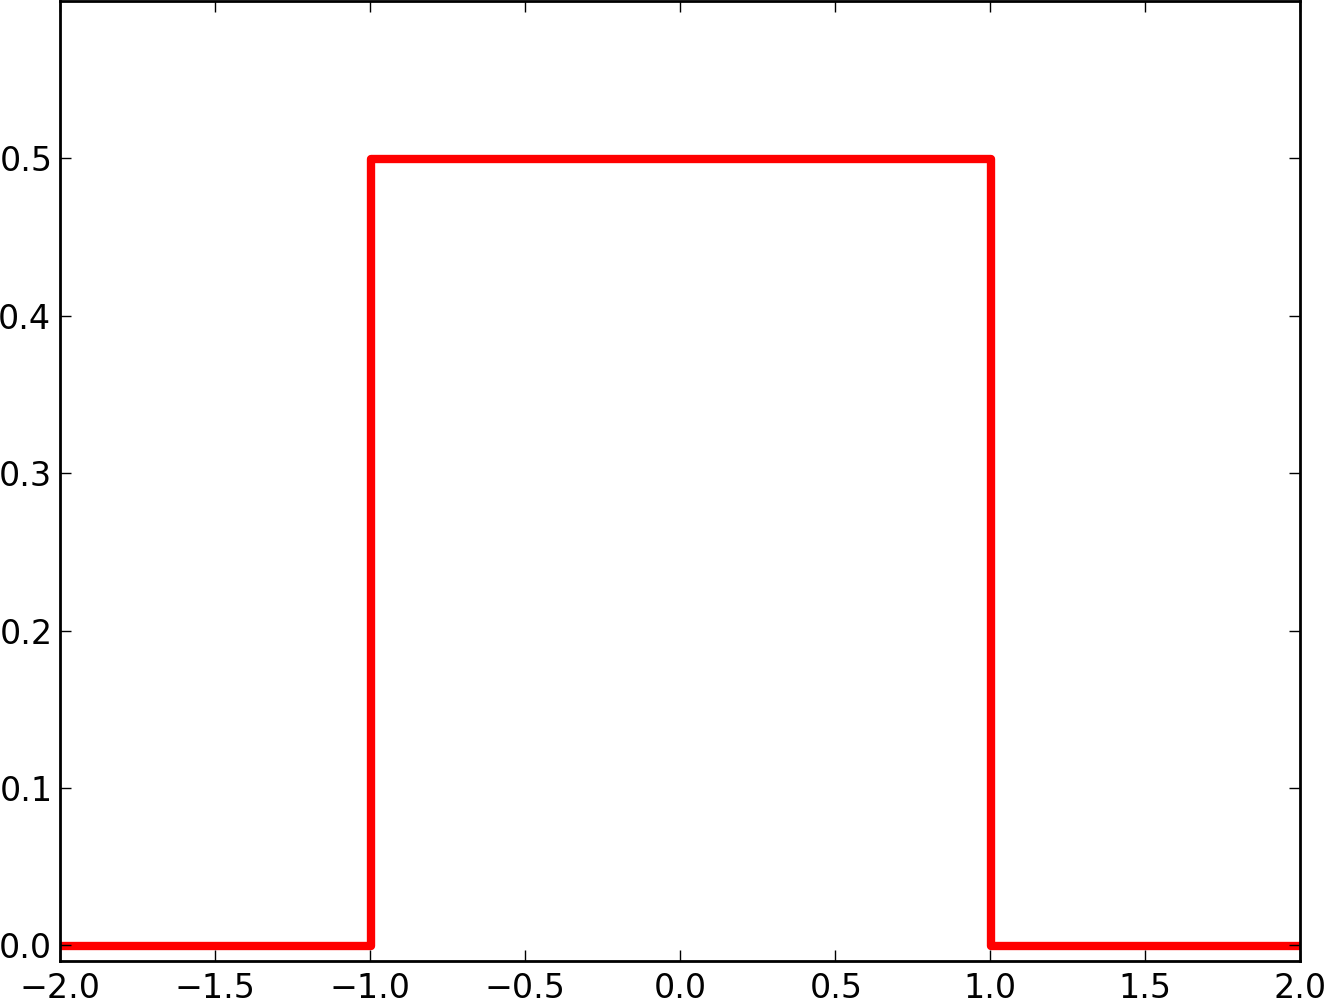
\includegraphics[width=0.9\textwidth]{./fig/fig_unif.png}
\caption{$a=-1$ and $b=1$}
\end{figure}
\end{exampleblock}
\end{columns}
\note{make basics calculations with uniform probability}

\end{frame}
%%%%%%%%%%%%%%%%%%%%%%%%%%%%%%%%%%%%%%%%%%%%%%%%%%%%%%%%%%%%%%%%%%%%%%%%%%%%%%%%%%%%%%
\begin{frame}{An example of joint probability}
Among 27 students who attend a class this day :
\begin{itemize}
\item 6 had a party last night and are still attentive in class 
\item 12 had a party last night and feel too sleepy to be attentive
\item 3 had no party last night but are not attentive in class
\item 6 had no party last night and are attentive in class
\end{itemize}

In term of Probability Mass Function:
\begin{itemize}
\item $N$ is a random variable such as $N=1$ if a random student did have a party and $0$ otherwise.
\item $A$ is a random variabl  suche as $A=1$ if a random student is attentive and $0$ otherwise.
\end{itemize}
\begin{table}
\centering
\begin{tabular}{|l||c|c|}
\hline
\backslashbox{N}{A} & 0 & 1 \\
\hline \hline
0 & 1/9 & 2/9 \\
\hline
1 & 4/9 & 2/9 \\
\hline
\end{tabular}
\end{table}
\note{Basic calculations (normalization), scheme}
\end{frame}

%%%%%%%%%%%%%%%%%%%%%%%%%%%%%%%%%%%%%%%%%%%%%%%%%%%%%%%%%%%%%%%%%%%%%%%%%%%%%%%%%%%%%%
\begin{frame}
\frametitle{Marginal probability}
\end{frame}


%%%%%%%%%%%%%%%%%%%%%%%%%%%%%%%%%%%%%%%%%%%%%%%%%%%%%%%%%%%%%%%%%%%%%%%%%%%%%%%%%%%%%%
\begin{frame}
\frametitle{Conditional probability}
\end{frame}


%%%%%%%%%%%%%%%%%%%%%%%%%%%%%%%%%%%%%%%%%%%%%%%%%%%%%%%%%%%%%%%%%%%%%%%%%%%%%%%%%%%%%%
\begin{frame}
\frametitle{Expectation, Variance, Covariance}
\end{frame}

%%%%%%%%%%%%%%%%%%%%%%%%%%%%%%%%%%%%%%%%%%%%%%%%%%%%%%%%%%%%%%%%%%%%%%%%%%%%%%%%%%%%%%
\begin{frame}
\frametitle{Gaussian Distribution}
\end{frame}

%%%%%%%%%%%%%%%%%%%%%%%%%%%%%%%%%%%%%%%%%%%%%%%%%%%%%%%%%%%%%%%%%%%%%%%%%%%%%%%%%%%%%%
\begin{frame}
\frametitle{Bayes' Rule}
\end{frame}


%%%%%%%%%%%%%%%%%%%%%%%%%%%%%%%%%%%%%%%%%%%%%%%%%%%%%%%%%%%%%%%%%%%%%%%%%%%%%%%%%%%%%%
\begin{frame}
\frametitle{Body's temperature and the magic of Bayes's rule}
\end{frame}



%%%%%%%%%%%%%%%%%%%%%%%%%%%%%%%%%%%%%%%%%%%%%%%%%%%%%%%%%%%%%%%%%%%%%%%%%%%%%%%%%%%%%%
\begin{frame}
\frametitle{Kullback-Leibler (KL) divergence}
\end{frame}



%%%%%%%%%%%%%%%%%%%%%%%%%%%%%%%%%%%%%%%%%%%%%%%%%%%%%%%%%%%%%%%%%%%%%%%%%%%%%%%%%%%%%%
\begin{frame}
\frametitle{An example}
\end{frame}


%%%%%%%%%%%%%%%%%%%%%%%%%%%%%%%%%%%%%%%%%%%%%%%%%%%%%%%%%%%%%%%%%%%%%%%%%%%%%%%%%%%%%%
\begin{frame}
\frametitle{Cross-entropy}
\end{frame}



%%%%%%%%%%%%%%%%%%%%%%%%%%%%%%%%%%%%%%%%%%%%%%%%%%%%%%%%%%%%%%%%%%%%%%%%%%%%%%%%%%%%%%
\begin{frame}
\frametitle{Sampling}
\begin{block}{Random sample (or independant identically distributed (i.i.d.) random variables)}
Considering a random variable $X$ following a probability distribution.

A \alert{sample}, is a set of $n$ independant random variables $\{X_1,X_2,\ldots,X_n\}$ such as 
each $X_i$ is following the same distribution as $X$.
\end{block}
\begin{block}{Observed values}
In practice, we have access to a particular realization of a random sample denoted
 $\{x_1,x_2,\ldots,x_n\}$
\end{block}
\end{frame}





\end{document}